\newpage
\section{Versuchsaufbau und -durchführung}
  In Abbildung \ref{fig:Aufbau} ist das Experiment schematisch dargestellt.
  \begin{figure}[h]
    \centering
    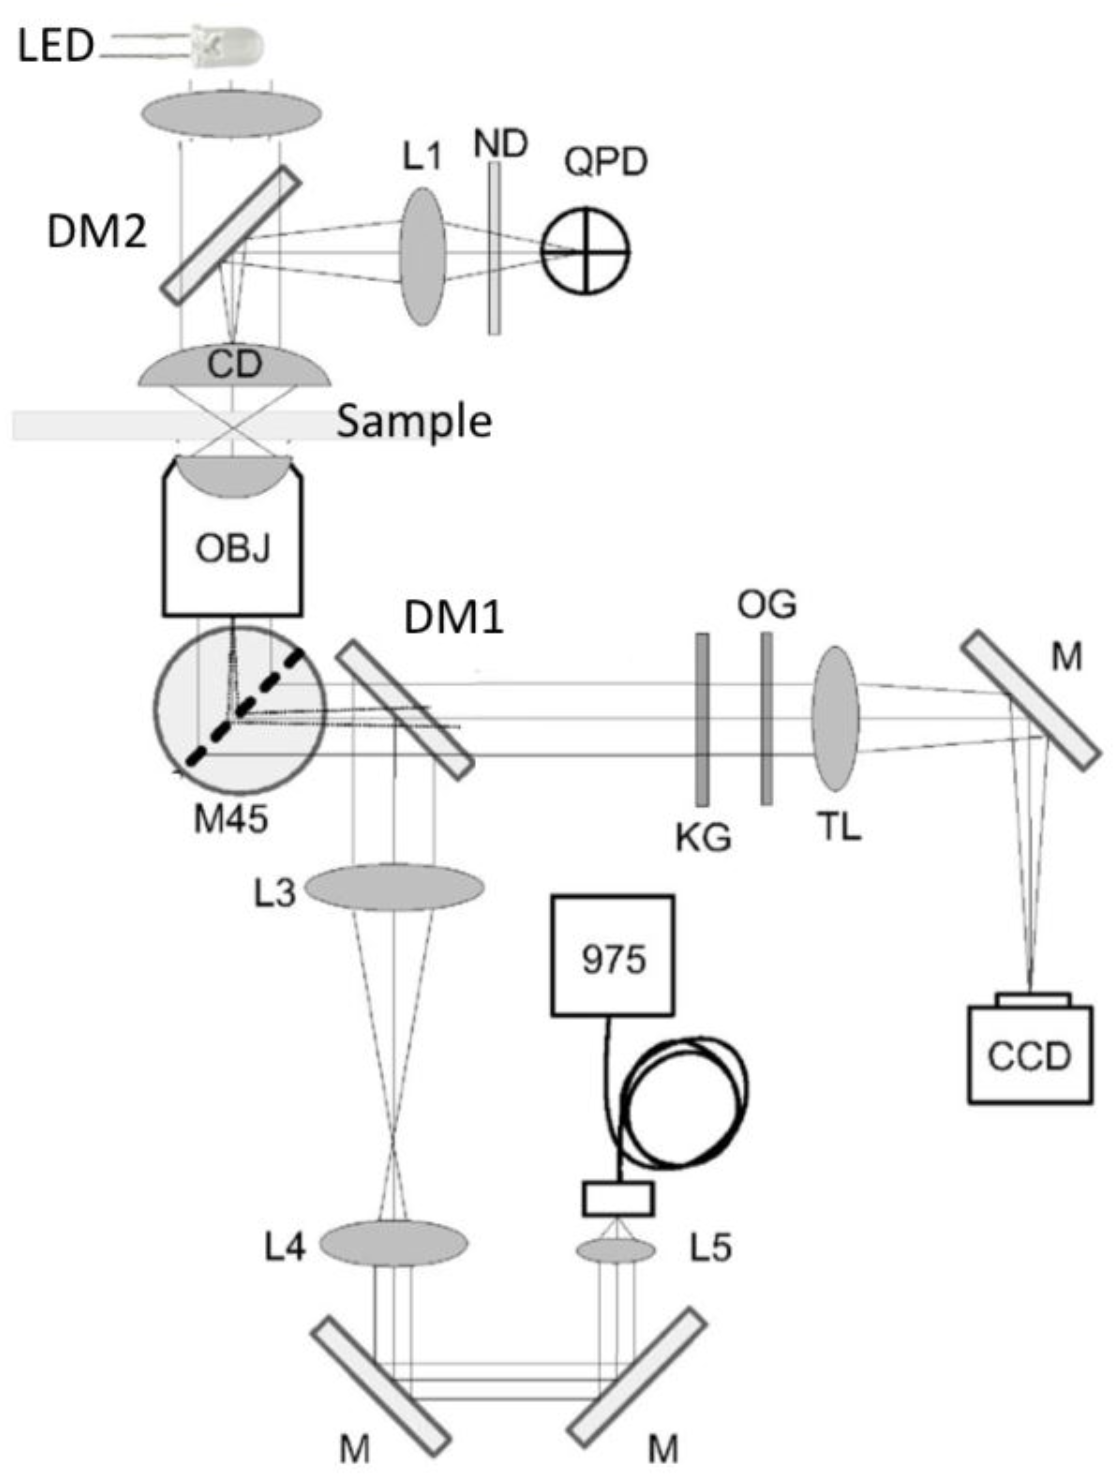
\includegraphics[width = 0.45\textwidth]{pictures/OPaufbau.png}
    \caption{Schematische Skizze des verwendeten Versuchsaufbaus. Entnommen aus \cite{tu_dortmund_versuchsanleitung_OptischePinzette}}
    \label{fig:Aufbau}
  \end{figure}
  Dieses besteht aus der optischen Pinzette und einem Lichtmikroskop, um die Probe während des Experiments beobachten zu können.
  Für die optische Pinzette wird ein $975\,\text{nm}$ Glasfaserlaser verwendet (975). Der Laserstrahl wird über verschiedene Linsen und Spiegel zu einem 100x Öl-Immersions-Objektiv (OBJ) gelenkt und auf die Probe fokussiert. Das transmittierte Licht wird durch ein weiteres Objektiv (CD) gesammelt und durch eine Viersegmentphotodiode (QPD) gemessen, welche es erlaubt, neben der Laserintensität ebenfalls die Position der Laserstrahls zu bestimmen. Um die Viersegmentphotodiode nicht zu übersättigen, passiert das Licht zuvor einen ND-Filter (ND).
  Für das Lichtmikroskop wird eine Weißlicht-LED (LED) verwendet. Der Strahlengang verläuft dabei entgegengesetzt zu dem des Lasers, also von oben nach unten durch die optische Pinzette, und wird von einer CCD-Kamera (CCD) aufgenommen.
  Um die Strahlen für die optische Falle und das Lichtmikroskop zu trennen werden zwei dichroitische Spiegel (DM1, DM2) eingesetzt, welche Licht abhängig von der Wellenlänge entweder transmittieren oder reflektieren.
  \subsection{Vorbereitung}
    Zuerst wird eine Quarzkügelchen-Probe in einem Objektträger mit Hilfe einer Pipette präpariert. Diese wird mit dem Lichtmikroskop untersucht, um die Pixelgröße der CCD-Kamera zu kalibrieren. Dann wird die optische Falle 'aktiviert', indem die Laserleistung aufgedreht wird, und ihre Position im beobachteten Bild bestimmt.
  \subsection{Kalibrierung der Viersegmentphotodiode}
  \label{sec:Kalib}
    Es wird eine neue Probe präpariert, diesmal in NaCl-haltigem Wasser, um die Beweglichkeit der Kugeln einzuschränken. Daraufhin wird ein Quarzkügelchen in die optische Falle plaziert und eine Positionskalibrierung, mit einer Scanlänge von $\SI{10}{\micro\metre}$ und 100 Schritten, durchgeführt für 5 verschiedene Laserleistungen ($\SI{4.83}{\milli\watt}$, $\SI{33.5}{\milli\watt}$, $\SI{63.4}{\milli\watt}$, $\SI{93.3}{\milli\watt}$, $\SI{123.2}{\milli\watt}$).
    Außerdem wurde durch eine Veränderung des z-Piezo-Stufenwerts die fokale Position der optischen Falle bis zu $\SI{250}{\micro\metre}$ variiert und das Diodensummensignal an der Viersegmentphotodiode gemessen.
  \subsection{Messungen zur Bestimmung der Fallensteifigkeit und Boltzmann-Konstante}
    Als Nächstes wird die \textit{force calibration} des Programms verwendet und damit das spektrale Leistungsspektrum aufgenommen. Das Ganze wird zuerst ohne externe Krafteinwirkung und dann mit einer externen Bewegung in x- und y-Richtung durchgeführt, auch hier wieder für 5 Werte der Laserleistung. Zum Schluss wird die Messung erneut wiederholt, diesmal mit einem eingesetzten Vortex-Retarder in den Strahlengang des Lasers.
    Der Fokus wird dabei die ganze Zeit über konstant gehalten und entspricht dem Fokus bei der Positionskalibrierung in \ref{sec:Kalib}.
  \subsection{Untersuchung von Vesikeln in Zwiebelzellen}
    Es wird eine Monolage aus dem Innern einer Zwiebel entfernt und auf einem Objektträger präpariert.
    Zuerst wird ein Vesikel gefunden und dessen Bewegungsmuster untersucht. Daraufhin werden unterschiedliche Vesikel eingefangen und untersucht. Die Bewegung der Organellen werden auf verschiedene Weisen manipuliert und die Ergebnisse in Bildschirmaufnahmen festgehalten.
    Als Nächstes wird ein Vesikel mit konstanter Geschwindigkeit untersucht mit dem Ziel dessen Größe und Geschwindigkeit zu charakterisieren.
    Zum Schluss wird die Laserleistung langsam erhöht und die Spannung an der Viersegmentphotodiode gemessen, bis das Vesikel die optische Falle nicht mehr überwinden kann.
    
    Jede 30 Minuten muss die Probe dabei erneuert werden, da die Lebenszeit einer Zwiebelzelle zeitlich sehr beschränkt ist.